% Editable reconstruction; interpretation recorded in root.json.
% Shared standalone design for the editable figure reconstructions.
\documentclass[tikz,border=5pt,10pt]{standalone}
\usepackage[T1]{fontenc}
\usepackage[utf8]{inputenc}
\usepackage{newpxtext,newpxmath}
\usepackage[scaled=.94]{sourcesanspro}
\usepackage{pgfplots}
\pgfplotsset{compat=1.18}
\usetikzlibrary{arrows.meta,calc,positioning,decorations.pathreplacing,
  decorations.markings,patterns,matrix,shapes.geometric,fit,backgrounds,
  intersections,angles,quotes}
\definecolor{ink}{HTML}{203746}
\definecolor{accent}{HTML}{146C78}
\definecolor{muted}{HTML}{667780}
\definecolor{signalred}{HTML}{B94B44}
\color{ink}
\tikzset{>=Latex,line width=.8pt,
  every node/.style={font=\small},
  axis/.style={->,draw=muted,line width=.5pt},
  guide/.style={draw=muted,dashed,line width=.45pt},
  curve/.style={draw=accent,line width=1pt},
  marker/.style={circle,fill=accent,inner sep=1.5pt},
  labelbox/.style={fill=white,inner sep=2pt}}

\begin{document}

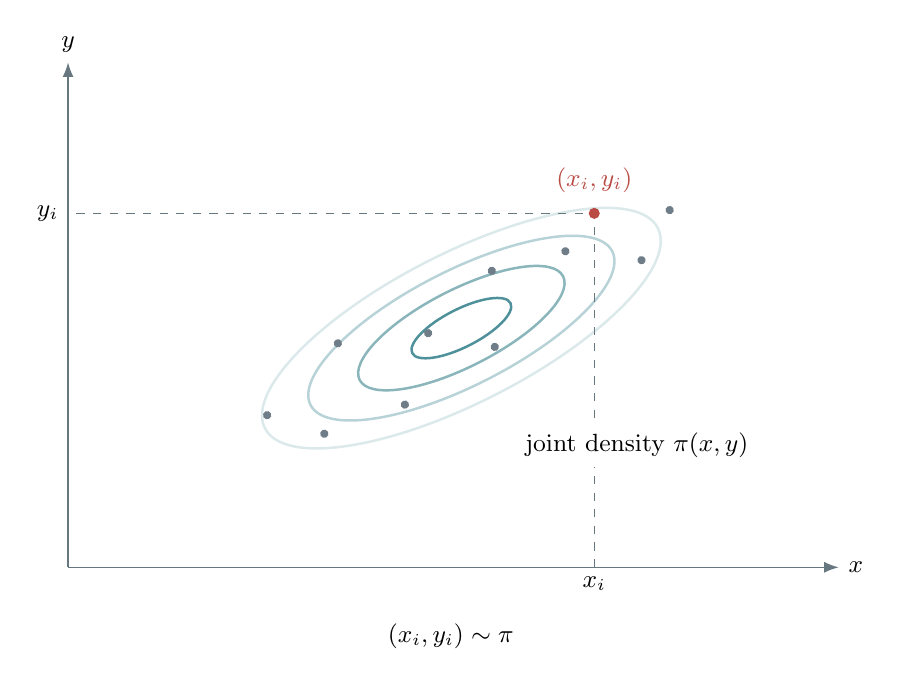
\begin{tikzpicture}[x=1.35cm,y=1.35cm]
\draw[axis] (-3.7,-2.25)--(3.55,-2.25) node[right] {$x$};
\draw[axis] (-3.7,-2.25)--(-3.7,2.5) node[above] {$y$};
\begin{scope}[rotate=27]
\foreach \a/\b/\col in {2.8/.95/accent!15,2.15/.73/accent!30,1.45/.49/accent!50,.7/.24/accent!75}{\draw[\col,line width=.9pt] (0,0) ellipse (\a cm and \b cm);}
\foreach \p in {(-2,.1),(-1.6,-.3),(-1.1,.4),(-.8,-.4),(-.3,.1),(.2,-.3),(.5,.35),(1.2,.2),(1.8,-.2),(2.25,.1)}{\fill[ink!65] \p circle(1.5pt);}
\end{scope}
\coordinate (sample) at (1.25,1.08);
\draw[guide] (1.25,-2.25)--(sample)--(-3.7,1.08);
\fill[signalred] (sample) circle(2pt) node[above=4pt] {$(x_i,y_i)$};
\node[below] at (1.25,-2.25) {$x_i$};\node[left] at (-3.7,1.08) {$y_i$};
\node[fill=white] at (1.65,-1.1) {joint density $\pi(x,y)$};
\node at (-.1,-2.9) {$(x_i,y_i)\sim\pi$};
\end{tikzpicture}
\end{document}
